\tp{Mesures de vitesses angulaires}

% TO DO : ins�rer figure

\vressort{1}


\begin{multicols}{2}

\objectifs{
\item mettre en �vidence une technique de mesure de vitesse angulaire
  utilisant l'�lectromagn�tisme.  % �lectromagn�tique ?
}

%\vressort{1}

\materiel{
\item oscilloscope et fiche BNC
\item fils
\item grande bobine
\item moteur � courant continu avec un aimant fix� sur le rotor
\item g�n�rateur de tension continu ajustable
}

\begin{center}
%\rule{7cm}{6cm}

\begin{figure}[H]
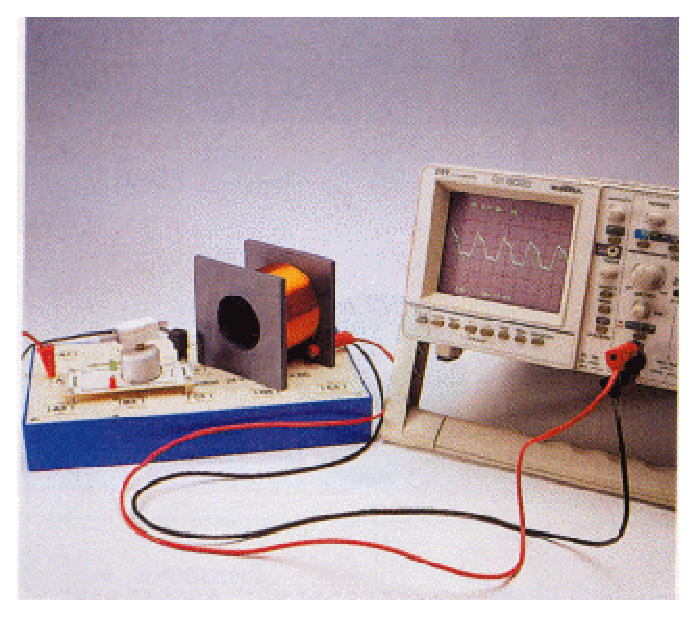
\includegraphics[width=9cm]{tp_prem_s_phys/tp03_rotation/tp_meca_rotation.gif.eps}
\caption{Dispositif exp�rimental}
\end{figure}
\end{center}

\end{multicols}


\vressort{3}

\section{Mesure � l'aide d'un aimant tournant}

\subsection{Principe}
Un aimant entra�n� par un moteur � courant continu tourne � vitesse
constante devant une bobine. Il se cr�e dans la bobine un courant
induit. On observe � l'aide d'un oscilloscope les variations de la
tension aux bornes de la bobine.

\subsection{Protocole}
\begin{itemize}
\item Fixer sur l'axe du moteur un aimant � 2 p�les.
\item Faire fonctionner le moteur afin que l'aimant tourne devant
  l'une des faces de la bobine conductrice reli�e � une voie de
  l'oscilloscope.
\item R�gler l'oscilloscope pour observer convenablement
  l'oscillogramme de la tension aux bornes de la bobine.
\end{itemize}


\vressort{3}

\section{Question}
\begin{enumerate}
\item Quelles sont les caract�ristiques de la tension aux bornes de la
  bobine ?
\item Modifier la tension d'alimentation du moteur � courant
  continu. Comment �voluent les caract�ristiques de la tension aux
  bornes de bobine ?
\item L'aimant comporte $p = 1$ paire de p�les (2 p�les). Quelle est la
  relation entre la p�riode de la tension mesur�e sur l'oscilloscope
  et la vitesse de rotation du moteur exprim�e en $tr.s^{-1}$ ?
\item Mesurer la vitesse de rotation du moteur pour diff�rentes
  tensions d'alimentation.
\item Rechercher le principe de fonctionnement d'une g�n�ratrice de
  bicyclette, improprement appel�e dynamo.
\end{enumerate}
